%% start of file `template.tex'.
%% Copyright 2006-2013 Xavier Danaux (xdanaux@gmail.com).
%
% This work may be distributed and/or modified under the
% conditions of the LaTeX Project Public License version 1.3c,
% available at http://www.latex-project.org/lppl/.


\documentclass[11pt,a4paper,roman]{moderncv}        % possible options include font size ('10pt', '11pt' and '12pt'), paper size ('a4paper', 'letterpaper', 'a5paper', 'legalpaper', 'executivepaper' and 'landscape') and font family ('sans' and 'roman')

% modern themes
\moderncvstyle{banking}                            % style options are 'casual' (default), 'classic', 'oldstyle' and 'banking'
\moderncvcolor{blue}                                % color options 'blue' (default), 'orange', 'green', 'red', 'purple', 'grey' and 'black'
%\renewcommand{\familydefault}{\sfdefault}         % to set the default font; use '\sfdefault' for the default sans serif font, '\rmdefault' for the default roman one, or any tex font name
%\nopagenumbers{}                                  % uncomment to suppress automatic page numbering for CVs longer than one page

% character encoding
\usepackage[utf8]{inputenc}
\usepackage{fontawesome}
\usepackage{tabularx}
\usepackage{ragged2e}
% if you are not using xelatex ou lualatex, replace by the encoding you are using
%\usepackage{CJKutf8}                              % if you need to use CJK to typeset your resume in Chinese, Japanese or Korean

% adjust the page margins
\usepackage[scale=0.8]{geometry}
\usepackage{multicol}
%\setlength{\hintscolumnwidth}{3cm}                % if you want to change the width of the column with the dates
%\setlength{\makecvtitlenamewidth}{10cm}           % for the 'classic' style, if you want to force the width allocated to your name and avoid line breaks. be careful though, the length is normally calculated to avoid any overlap with your personal info; use this at your own typographical risks...

\usepackage{import}

\usepackage{graphicx}
\usepackage{tikz}
\usepackage{tikzpagenodes}
\usetikzlibrary{calc} 
\usepackage[inline]{enumitem}
\usepackage{amsmath}


% personal data
\name{Sajjad P.}{Savoji}
% \title{Curriculum Vitae}                               % optional, remove / comment the line if not wanted
%\address{Gholhak , Tehran , Iran }{}{}% optional, remove / comment the line if not wanted; the "postcode city" and and "country" arguments can be omitted or provided empty
% \phone[mobile]{909-839-3097}                   % optional, remove / comment the line if not wanted
% \phone[fixed]{01234 123456}                    % optional, remove / comment the line if not wanted
%\phone[fax]{+3~(456)~789~012}                      % optional, remove / comment the line if not wanted
% \email{xpan1@swarthmore.edu}                               % optional, remove / comment the line if not wanted
% \homepage{shawnpan.me}                         % optional, remove / comment the line if not wanted
% \extrainfo{}                 % optional, remove / comment the line if not wanted
%\photo[64pt][0.4pt]{picture}                       % optional, remove / comment the line if not wanted; '64pt' is the height the picture must be resized to, 0.4pt is the thickness of the frame around it (put it to 0pt for no frame) and 'picture' is the name of the picture file
%\quote{Some quote}                                 % optional, remove / comment the line if not wanted

% to show numerical labels in the bibliography (default is to show no labels); only useful if you make citations in your resume
%\makeatletter
%\renewcommand*{\bibliographyitemlabel}{\@biblabel{\arabic{enumiv}}}
%\makeatother
%\renewcommand*{\bibliographyitemlabel}{[\arabic{enumiv}]}% CONSIDER REPLACING THE ABOVE BY THIS

% bibliography with mutiple entries
%\usepackage{multibib}
%\newcites{book,misc}{{Books},{Others}}
  
\newcommand*{\customcventry}[7][.25em]{
  \begin{tabular}{@{}l} 
    {\bfseries #4}
  \end{tabular}
  \hfill% move it to the right
  \begin{tabular}{l@{}}
     {\bfseries #5}
  \end{tabular} \\
  \begin{tabular}{@{}l} 
    {\itshape #3}
  \end{tabular}
  \hfill% move it to the right
  \begin{tabular}{l@{}}
     {\itshape #2}
  \end{tabular}
  \ifx&#7&%
  \else{\\%
    \begin{minipage}{\maincolumnwidth}%
      \small#7%
    \end{minipage}}\fi%
  \par\addvspace{#1}}

\newcommand*{\customcvproject}[4][.25em]{
%   \vfill\noindent
  \begin{tabular}{@{}l} 
    {\bfseries #2}
  \end{tabular}
  \hfill% move it to the right
  \begin{tabular}{l@{}}
     {\itshape #3}
  \end{tabular}
  \ifx&#4&%
  \else{\\%
    \begin{minipage}{\maincolumnwidth}%
      \small#4%
    \end{minipage}}\fi%
  \par\addvspace{#1}}

\setlength{\tabcolsep}{12pt}

%----------------------------------------------------------------------------------
%            content
%----------------------------------------------------------------------------------
\begin{document}
	\begin{minipage}[t]{0.2 \textwidth}
		\hspace*{0.4cm}
		\begin{tikzpicture}[baseline=(ola.center),inner sep=0pt]
		\clip (0,0)  circle (2cm) node (ola) {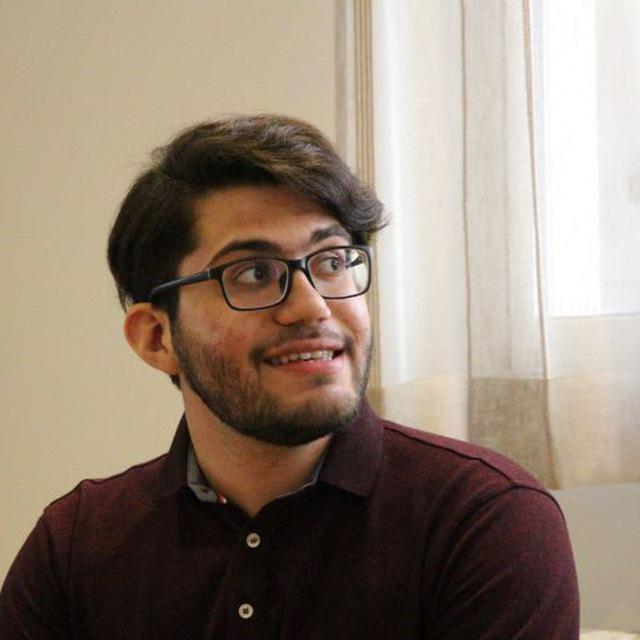
\includegraphics[width=4cm]{resumepic.jpg}};
		\end{tikzpicture}
	\end{minipage}
	\hfill
	\begin{minipage}[t]{0.73\textwidth}
		\makecvtitle
		\vspace*{-23mm}
		\begin{center}
			\begin{tabular}{ c c c }
				 \href{mailto:sj.pakdaman@ut.ac.ir}{\faEnvelopeO\enspace sj.pakdaman@ut.ac.ir} &  \href{https://gitlab.com/sj.pakdaman}{\faGitlab\enspace sj.pakdaman} &  \faMobile\enspace 0098-919-591-9545\\  
			\end{tabular}
			\vspace*{-100mm}
		 Gholhak,Tehran Province,Iran
		\end{center}
	\end{minipage} 
%\begin{CJK*}{UTF8}{gbsn}                          % to typeset your resume in Chinese using CJK
%-----       resume       ---------------------------------------------------------


\section{Education}
{\customcventry{}{B.S.c in Electrical Engineering , Major in Communication Systems , Minor in Computer Engineering}{University of Tehran}{}{}{}}
\begin{itemize}
	\item EE Cumulative GPA: 17.69 / 20
	\item CE Cumulative GPA: 18.88 / 20 (Class rank: 2)
\end{itemize}

{\customcventry{}{Diploma in Mathematics and Physics}{NODET Allameh Helli 8 Branch}{}{}{}}
National Organization for Development of Exceptional Talents AKA "NODET"
\begin{itemize}
	\item GPA: 19.73 / 20
\end{itemize}

\subsection{Research Interest}
Deep Learning, Computer Networks, Information Theory, Source Coding, Massive MIMO, 5G and cellular communication, Object Localization, Artificial Intelligence, Reinforcement Learning, Optimization, Neural Networks.


\subsection{Selected Courses}
		Pattern Recognition,
		Neural Networks and Deep Learning, 
		Artificial Intelligence, 
		Digital Communication Systems, 
		Digital Signal Processing, 
		Communication Systems , 
		Linear Algebra, 
		Statistics and Probability, 
		Operating Systems, 
		Advance Programming, 
		Data Structure, 
		Linear Control Systems, 
		Realtime Digital Processing Lab, 
		Digital Communication Lab. 
\section{Awards and Achievements}
\begin{minipage}{\maincolumnwidth}%
	\small{
		\begin{itemize}
			\item $3^{rd}$place in Iran and $93^{th}$ place worldwide in IEEExtreme 11.0 from 2121 teams.
			\item $8^{th}$ place in Iran and $733^{th}$ place worldwide in IEEExtreme 12.0 from 3358 teams. 
			\item Gold medalist(2016) and silver medalist(2017) basketball player in University of Tehran sport festival.
			\item Gold medalist in city of Tehran 2014 student sport competition.
	\end{itemize}}%
\end{minipage}%

\section{Experience}

\begin{itemize}
		\item \textbf{IEEExtreme 12, 13 and 14 ambassador (International volunteer work)} \hfill {April 2018 - Agust 2020}
		\item \textbf{IEEE Data Science Winter School Mentorship} \hfill {January 2020}
		\item \textbf{RA in computer networks lab at university of tehran} \hfill {Agust 2019 - Agust 2020}
		\item \textbf{Vice Chair of IEEE University of Tehran student branch} \hfill {April 2018 - April 2019}
		\item \textbf{Summer Internship in Secure Communication Lab} \hfill {June 2019 - September 2019}
		\item \textbf{IEEEmadC ambassador (International volunteer work)} \hfill {April 2018 - November 2019}

\end{itemize}

% {\customcventry{April 2018 - April 2019}{}{Vice Chair of IEEE University of Tehran student branch}{}{}
% {
% 	% \begin{itemize}
%     % \item The Student Branch Vice-Chair is the junior Executive Officer. He/she should help the Branch Chair with the workload, oversee some of the subcommittees, and manage some of the activities throughout the semester.
% 	% \end{itemize}
% }

% {\customcventry{June - September 2019}{}{Summer Internship in Secure Communication Lab}{University of Tehran}{}
% {
% 	% \begin{itemize}
%   	% \item Secure Communication Lab in UofT is a leading lab in which real-life problems are addressed using AI/Deep Learning techniques. Through this reasearch internship I developed several Artificial Neural Networks such as YOLO2 , LSTM , CNN and MLP. My task was to build a translator from Iranian Sign Language to written words.  
% 	% \end{itemize}
% }

% {\customcventry{January 2020}{}{IEEE Data Science Winter School Mentorship}{University of Tehran}{}
% {
% 	% \begin{itemize}
%   	% \item DSWS(Data Science Winter School) is an evet held at UTSB in which participants gain general knowledge regarding Statistical Inference, ML, DeepLearning, etc. I contributed both as an instructor and a hands-on designer. 
% 	% \end{itemize}
% }

% {\customcventry{April 2018 - November 2019}{}{IEEExtreme 12.0 and 13.0 ambassador}{International volunteer work}{}
% {
% 	% \begin{itemize}
% 	% 	\item IEEEXtreme is an annual hackathon and competitive programming challenge in which teams of IEEE Student members compete in a 24-hour time span against each other to solve a set of programming problems.
% 	% 	\item An ambassador's job is to encourage students to participate the challenge.
% 	% \end{itemize}
% }	
% }

% {\customcventry{April 2018 - November 2019}{}{IEEEmadC ambassador}{International volunteer work}{}
% {
% 	% \begin{itemize}
% 	% 	\item IEEEmadC (Mobile Applications Development Contest) is an international contest organized by volunteers for IEEE student members across the globe. The main goal is to educate and encourage students to pursue their future career as mobile application developers.
% 	% 	\item An ambassador's job is to encourage students to participate the challenge.
% 	% \end{itemize}
% }	
% }


\section{Educational Experience}
\begin{itemize}
		\item \textbf{Pattern Recognition TA} \hfill {Spring 2020}
		\item \textbf{Digital Signal Processing TA} \hfill {Spring 2020}
		\item \textbf{Communication Systems I TA} \hfill {Fall 2019, Spring 2020}
		\item \textbf{Engineering Probability and Statistics TA}  \hfill {Spring 2019, Fall 2019}
		\item \textbf{Electronics I TA} \hfill {Spring 2018}
\end{itemize}

\section{Key Skills}
	\begin{minipage}[t]{0.5 \textwidth}
		\subsection{Programming Languages}
		\begin{itemize}
			\item Python (numpy, pandas, sklean, pytorch)
			\item C++ (Advanced)
			\item C (Advanced)
			\item System Verilog
			\item R Language
			\item HTML5, JS, CSS, Bootstrap 
		\end{itemize}
	\end{minipage}
	\begin{minipage}[t]{0.5 \textwidth}
		\subsection{Platorms}
		\begin{itemize}
			\item Jupyter Notebook and Google Colaboratory
			\item MATLAB Simulink \& toolboxes
			\item Hardware simulators: Modelsim , Quartus 
			\item Circuit simulators: Multisim
			\item Micro controller simulators: Proteus,Codevision
			\item \LaTeX, Microsoft Word
		\end{itemize}
	\end{minipage}
	\subsection{Digital Devices and Microcontrollers}
		\begin{itemize*}
			\item {FPGA}  \hfill 
			\item {DSPs} \hfill 
			\item {AVR ATmeg series} \hfill 
			\item {Raspberry Pi 2,3} \hfill
			\item {Arduino} \hfill
		\end{itemize*}	


\section{Academic Projects}
{\customcvproject{ \href{https://gitlab.com/sj.pakdaman/vae}{Vriational Autoencoder} \href{https://gitlab.com/sj.pakdaman/vae}{\textcolor{blue}{(link)}}  }{August 2020}
	{\begin{itemize}
			\item A CNN model was trained to serve as a VAE. This model was tested on MNIST dataset.
			% \item In the first branch some new features were added to the console and terminal.
			% \item The second branch adds some new system calls to the XV6 kernel.
			% \item In the third branch multiple CPU scheduling algorithms support was added.
			% \item In the fourth branch process synchronization memory barrier was implemented.
			% \item The last branch is about memory and paging of XV6. XV6 does not handle demand paging.We added paging to XV6 then we added different paging algorithms such as LRU, NFU, Clock, FIFO.
		\end{itemize}
	}
}

{\customcvproject{ \href{https://gitlab.com/sj.pakdaman/dcgan}{DCGAN} \href{https://gitlab.com/sj.pakdaman/dcgan}{\textcolor{blue}{(link)}}  }{August 2020}
	{\begin{itemize}
			\item A deep concolutional genarative adversial networks was trained on the CIFAR10 dataset.
			% \item In the first branch some new features were added to the console and terminal.
			% \item The second branch adds some new system calls to the XV6 kernel.
			% \item In the third branch multiple CPU scheduling algorithms support was added.
			% \item In the fourth branch process synchronization memory barrier was implemented.
			% \item The last branch is about memory and paging of XV6. XV6 does not handle demand paging.We added paging to XV6 then we added different paging algorithms such as LRU, NFU, Clock, FIFO.
		\end{itemize}
	}
}

{\customcvproject{ \href{https://gitlab.com/sj.pakdaman/cgan-and-acgan}{CGAN and ACGAN} \href{https://gitlab.com/sj.pakdaman/cgan-and-acgan}{\textcolor{blue}{(link)}}  }{August 2020}
	{\begin{itemize}
			\item An Auxiliary classifier genarative adversial networks was trained on the CIFAR10 dataset.
			% \item In the first branch some new features were added to the console and terminal.
			% \item The second branch adds some new system calls to the XV6 kernel.
			% \item In the third branch multiple CPU scheduling algorithms support was added.
			% \item In the fourth branch process synchronization memory barrier was implemented.
			% \item The last branch is about memory and paging of XV6. XV6 does not handle demand paging.We added paging to XV6 then we added different paging algorithms such as LRU, NFU, Clock, FIFO.
		\end{itemize}
	}
}

% {\customcvproject{\href{https://gitlab.com/sj.pakdaman/ap_drive}{AP Drive} \href{https://gitlab.com/sj.pakdaman/ap_drive}{\textcolor{blue}{(link)}}}{September 2018 - January 2019}
%   {\begin{itemize}
%     \item A File Hosting Service inspired by Drop Box using C++ with a web based GUI
%     % \item Allows multi-user synchronization , file sharing as group and individual, file management, upload and download and storage management for root and admin users. All features are accessible both locally and through the Internet. 
%     % \item this project was implemented by Object Oriented and multi-file methodology
%     % \item phase1: Program works similar to linux file system. Implemented locally and without graphical features.
%     % \item phase2: User interface implementation based on Client-Server distributed model by using web tools.
%   \end{itemize}
%   }
% }


% {\customcvproject{\href{https://gitlab.com/sj.pakdaman/kingdomrush}{Kingdom Rush}}{September 2018 - January 2019}
% {\begin{itemize}
%   \item a real time tower defense game implemented by Simple DirectMedia Layer(SDL) graphical library using C++
%   \item the goal of this project was practicing Top-Down design programming methodology
%   \item this project was implemented by Object Oriented and multi-file methodology
% \end{itemize}
% }
% }

{\customcvproject{ \href{https://gitlab.com/sj.pakdaman/xv6}{XV6 development} \href{https://gitlab.com/sj.pakdaman/xv6}{\textcolor{blue}{(link)}}  }{January 2020}
	{\begin{itemize}
			\item This project is based on the XV6 operating system developed in MIT University. Each branch of this project is an adds a feature or improves the original XV6 kernel.
			% \item In the first branch some new features were added to the console and terminal.
			% \item The second branch adds some new system calls to the XV6 kernel.
			% \item In the third branch multiple CPU scheduling algorithms support was added.
			% \item In the fourth branch process synchronization memory barrier was implemented.
			% \item The last branch is about memory and paging of XV6. XV6 does not handle demand paging.We added paging to XV6 then we added different paging algorithms such as LRU, NFU, Clock, FIFO.
		\end{itemize}
	}
}

{\customcvproject{\href{https://gitlab.com/sj.pakdaman/voice_identification}{Voice Recognition using MLP} \href{https://gitlab.com/sj.pakdaman/voice_identification}{\textcolor{blue}{(link)}}  }{April 2019}
	{\begin{itemize}
			\item In this project a neural network was trained on the melfrequency coeficients of indivisual's voices to provide an identification systerm based on speech processing.  
		\end{itemize}
	}
}

{\customcvproject{\href{https://gitlab.com/sj.pakdaman/siamese}{Face Detection using CNNs}   \href{https://gitlab.com/sj.pakdaman/siamese}{\textcolor{blue}{(link)}}    }{July 2019}
	{\begin{itemize}
			\item the goal was to build a Convolutional NN using which the problem proposed by AT\&T faces dataset could be solved. To do so, the siamese network alongside with triple-loss cost function were used.
		\end{itemize}
	}
}

{\customcvproject{\href{https://gitlab.com/sj.pakdaman/fish_localization}{Object Localization}   \href{https://gitlab.com/sj.pakdaman/fish_localization}{\textcolor{blue}{(link)}}  }{July 2019}
	{\begin{itemize}
			\item This project is a simple implementation of YOLO2 network trained on the dataset proposed by \href{https://www.kaggle.com/c/the-nature-conservancy-fisheries-monitoring}{kaggle.com} to localize and identify different fish.
		\end{itemize}
	}
}

{\customcvproject{\href{https://gitlab.com/sj.pakdaman/humpback_whale}{Humpback Whale Identification}  \href{https://gitlab.com/sj.pakdaman/humpback_whale}{\textcolor{blue}{(link)}} }{July 2019}
	{\begin{itemize}
			\item The goal was to build a Convolutional NN using which the problem proposed by \href{https://www.kaggle.com/c/humpback-whale-identification}{kaggle} could be solved. To do so, the siamese network alongside with triple-loss cost function were used.
		\end{itemize}
	}
}

{\customcvproject{\href{https://gitlab.com/sj.pakdaman/asl_resnet101}{Transfer Learning for ASL}   \href{https://gitlab.com/sj.pakdaman/asl_resnet101}{\textcolor{blue}{(link)}}  }{July 2019}
	{\begin{itemize}
			\item This project was a prototype for American Sign Language(ASL) translation, in which few layers of Resnet101 was retrained on the data set provided from \href{https://www.kaggle.com/grassknoted/asl-alphabet}{kaggle.com}.
		\end{itemize}
	}
}


{\customcvproject{Smart House}{Jun 2018 – August 2018}
{\begin{itemize}
  \item IOT based project tested on a wooden home prototype using mostly Python and Java
%   \item Using a Raspberry Pi as central gateway of sensor communications, home daily activities such as opening doors, powering lights and watering flowers were done automatically.
%   \item Then the Raspberry Pi interacted through HTTPS and MQTT protocols with a simple Android app. As the Raspberry had massive computation capacity, vital warnings could activate edge computing services such as the fire extinguisher.
%   \item All sensory data was stored in thingtalk.ir platform and allowed us to provide user with cloud computing services such as graphs and data analysis  
\end{itemize}
}

{\customcvproject{\href{https://gitlab.com/sj.pakdaman/analog_modulatio_am_dsb_ssb}{Amplitude Modulations}    \href{https://gitlab.com/sj.pakdaman/analog_modulatio_am_dsb_ssb}{\textcolor{blue}{(link)}}  }{July 2019}
	{\begin{itemize}
			\item In this project several amplitude modulations such as AM , DSB and SSB were simulted in MATLAB.
			% \item In addition to demodulations, the so known syncronization problem that exists in synchronous demodulators were examined.
			% \item The result was that DSB modulation is less sensative to freq error. 
		\end{itemize}
	}
}



% {\customcvproject{git}{October 2016 - November 2016}
% 	{\begin{itemize}
% 			\item a simple distributed version-control system for tracking changes in source code during software development which basically works similar to linux git using C 
% 			\item working with multi dimensional pointers and dynamic memory allocation was the goal of project. 
% 		\end{itemize}
% 	}
% }

% {\customcvproject{Encryption}{June 2017 - July 2017}
% 	{\begin{itemize}
% 			\item encrypting short text symbols in color values of pixels using C++
% 			\item text characters was placed in pixels which had the most variance among it's neighbor pixels  
% 		\end{itemize}
% 	}
% }

% {\customcvproject{Noise removal}{January 2018 - February 2018}
% 	{\begin{itemize}
% 			\item removing noise of a .wav file using matlab
% 			\item first noise was detected and removed by Fourier analysis then using matlab FDA tool a more efficient filter was designed which removed noise perfectly.  
% 		\end{itemize}
% 	}
% }


{\customcvproject{Frequency Spectrum Analyzer}{January 2019 - February 2019}
	{\begin{itemize}
			\item A real-time frequency spectrum analyzer using C and AVR ATmeg series.
			% \item Surrounding voice was sampled using AVR's ADC module then using Fast Fourier Transform algorithm, frequency spectrum of voice was shown in an LED array.
			% \item To assure that hardware was working fine ,sampled data was transmitted to laptop using avr USART and frequency spectrum was double checked in matlab.
		\end{itemize}
	}
}

{\customcvproject{Real-time DC Motor Speed Estimation Using Optocounter}{January 2020}
	{\begin{itemize}
			% \item This project was a part of Electrical Machines Lab course taught at UofT.
			\item The goal was to build a device to estimate motor's speed using AVR and IR sensor.
		\end{itemize}
	}
}

{\customcvproject{More projects are available in my \href{https://gitlab.com/sj.pakdaman}{\textcolor{blue}{(Git repository)}}  }{}
	{
	}
}



% {\customcvproject{Online Store}{September 2018 - January 2019}
% 	{\begin{itemize}
% 			\item modeling a virtual store to manage trades and transactions of goods using C++
% 			% \item this project was implemented by Object Oriented and multi-file methodology
% 			\item The app provided user with special features such as discount offers , receipts and searching for different features of goods such as price , kind ,etc. 
% 		\end{itemize}
% 	}
% }
% }

% \section{MEMBERSHIPS}
% \begin{itemize}
	
% 	\noindent
% 	\parbox[t]{.6\textwidth}{\raggedright
% 		\item IEEE student member}\hfill
% 	\parbox[t]{.1\textwidth}{\centering
% 	}\hfill
% 	\parbox[t]{.3\textwidth}{\raggedleft
% 		September 2017 - present}%
% \end{itemize}

% Publications from a BibTeX file without multibib
%  for numerical labels: \renewcommand{\bibliographyitemlabel}{\@biblabel{\arabic{enumiv}}}% CONSIDER MERGING WITH PREAMBLE PART
%  to redefine the heading string ("Publications"): \renewcommand{\refname}{Articles}
%\nocite{*}
%\bibliographystyle{plain}
%\bibliography{publications}                        % 'publications' is the name of a BibTeX file

% Publications from a BibTeX file using the multibib package
%\section{Publications}
%\nocitebook{book1,book2}
%\bibliographystylebook{plain}
%\bibliographybook{publications}                   % 'publications' is the name of a BibTeX file
%\nocitemisc{misc1,misc2,misc3}
%\bibliographystylemisc{plain}
%\bibliographymisc{publications}                   % 'publications' is the name of a BibTeX file

%-----       letter       ---------------------------------------------------------

\end{document}


%% end of file `template.tex'.